\chapter{Regression, QR, and Numerical Stability}
\label{ch:regression-qr-stability}

\section{Regression Is Linear Algebra After Choosing Features}

Polynomial regression sounds nonlinear because polynomials contain powers such
as $t^2$ and $t^5$. But once the sample points are fixed, fitting the
coefficients is a linear problem.

Suppose we have data
\[
  (t_1,y_1),\ldots,(t_m,y_m)
\]
and want a degree-$d$ polynomial
\[
  p(t)=c_0+c_1t+c_2t^2+\cdots+c_dt^d.
\]
The unknowns are the coefficients
\[
  c=(c_0,\ldots,c_d)^T.
\]
The equations $p(t_i)=y_i$ form
\[
  Xc=y,
\]
where
\[
  X=
  \begin{bmatrix}
  1&t_1&t_1^2&\cdots&t_1^d\\
  1&t_2&t_2^2&\cdots&t_2^d\\
  \vdots&\vdots&\vdots&&\vdots\\
  1&t_m&t_m^2&\cdots&t_m^d
  \end{bmatrix},
  \qquad
  y=\begin{bmatrix}y_1\\ \vdots\\ y_m\end{bmatrix}.
\]
This is a Vandermonde feature matrix. Its columns are features evaluated at
the observed input values:
\[
  1,\quad t,\quad t^2,\quad \ldots,\quad t^d.
\]

\begin{figure}[htbp]
  \centering
  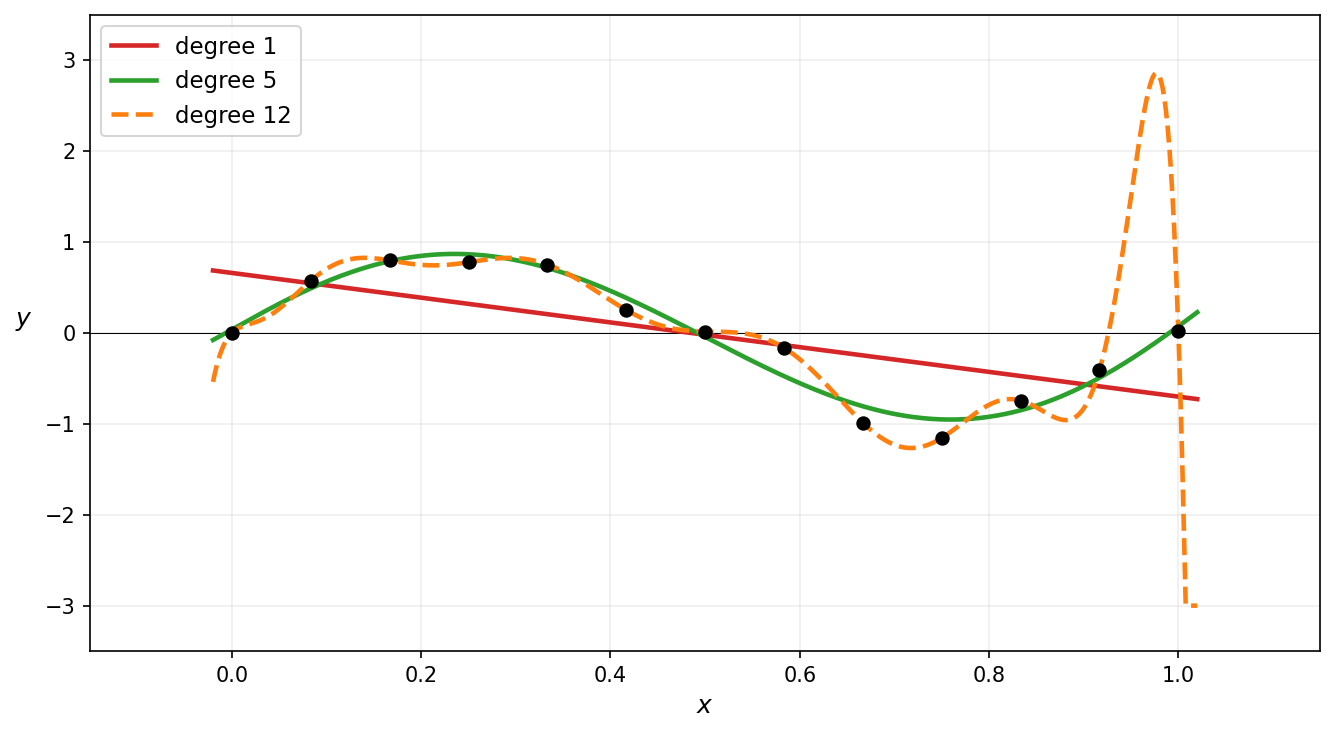
\includegraphics[width=0.88\textwidth]{book/assets/figures/core/fig05_poly_regression.png}
  \caption{Polynomial regression can underfit, fit reasonably, or overfit.
  The linear algebra is the same in each case; the feature choice changes the
  column space where the data vector is projected.}
\end{figure}

\begin{aimlbox}
Regression is not introduced here as ``the linear algebra of AI.'' It is a
clean example of a broader lesson: after choosing features, many data-fitting
tasks ask for the closest point in a column space. That is the part of the
story this book needs.
\end{aimlbox}

\section{Training Error And Validation Error}

The least-squares solution minimizes the training error
\[
  \norm{Xc-y}
\]
on the observed data. As the polynomial degree grows, the column space of $X$
usually grows, so training error cannot increase.

That does not mean the model is better. A high-degree polynomial can chase
noise and behave poorly between or beyond the sampled points. To detect this,
we compare training error with validation error: error on new data not used to
fit the coefficients.

\begin{warningbox}
Low training error is a linear-algebraic fact about projection onto a larger
subspace. Good prediction is a modeling question. Linear algebra explains the
geometry of the fit; it does not by itself decide which model is appropriate.
\end{warningbox}

\section{Normal Equations Revisited}

The normal equations for the regression problem are
\[
  X^TX\hat{c}=X^Ty.
\]
If the columns of $X$ are independent, then
\[
  \hat{c}=(X^TX)^{-1}X^Ty.
\]
This formula is mathematically useful and often appears in derivations. It
also exposes a numerical problem: $X^TX$ may be much worse conditioned than
$X$.

\begin{definition}[Condition number, informal]
The condition number of an invertible matrix measures how much relative input
error can be amplified in the output. Large condition numbers mean small
rounding or measurement errors can become large changes in the computed
answer.
\end{definition}

For least-squares problems, forming $X^TX$ often roughly squares the condition
number. If $X$ is already ill-conditioned, the normal equations can lose many
digits of accuracy.

\section{Orthogonal Bases And Gram--Schmidt}

The numerical issue suggests a better goal: instead of working with arbitrary
columns of $X$, replace them with orthonormal columns spanning the same column
space.

\begin{definition}[Orthonormal list]
Vectors $q_1,\ldots,q_k$ are \emph{orthonormal} if
\[
  \inner{q_i}{q_j}=
  \begin{cases}
  1,&i=j,\\
  0,&i\neq j.
  \end{cases}
\]
\end{definition}

If $Q$ has orthonormal columns, then
\[
  Q^TQ=I.
\]
Projection onto $\col(Q)$ is especially simple:
\[
  \Proj_{\col(Q)}(b)=QQ^Tb.
\]

\begin{figure}[htbp]
  \centering
  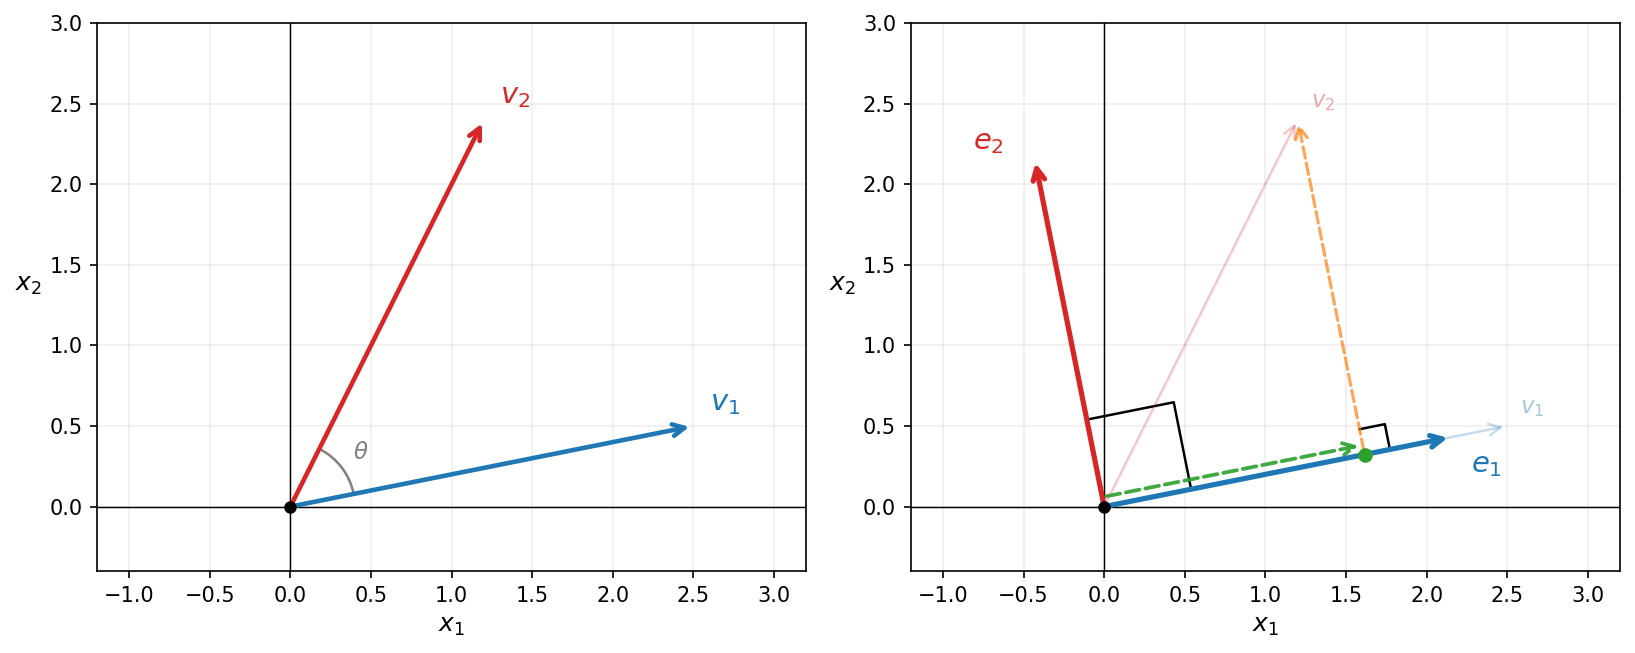
\includegraphics[width=0.90\textwidth]{book/assets/figures/core/fig06_gram_schmidt.png}
  \caption{Gram--Schmidt subtracts projections. The first vector determines
  the first direction; the second contributes only its residual perpendicular
  to the first.}
\end{figure}

\begin{theorem}[Gram--Schmidt]
Let $v_1,\ldots,v_k$ be linearly independent vectors in an inner product
space. Define
\[
  u_1=v_1,\qquad q_1=\frac{u_1}{\norm{u_1}},
\]
and for $j=2,\ldots,k$,
\[
  u_j
  =
  v_j-\sum_{i=1}^{j-1}\inner{v_j}{q_i}q_i,
  \qquad
  q_j=\frac{u_j}{\norm{u_j}}.
\]
Then $q_1,\ldots,q_k$ is an orthonormal basis for
$\Span(v_1,\ldots,v_k)$.
\end{theorem}

\begin{proof}
At step $j$, the vector $u_j$ is obtained from $v_j$ by subtracting the part of
$v_j$ lying in the span of the earlier $q_i$'s. Therefore $u_j$ is orthogonal
to each earlier $q_i$. Since $v_j$ is not in the span of the previous vectors,
$u_j\neq 0$, so normalization is allowed. The span is unchanged because each
$u_j$ is built from $v_1,\ldots,v_j$, and each $v_j$ can be recovered from
$u_j$ plus earlier $q_i$'s.
\end{proof}

\section{QR Factorization}

Apply Gram--Schmidt to the columns of a full-column-rank matrix
$A\in\R^{m\times n}$. The result is
\[
  A=QR,
\]
where
\[
  Q\in\R^{m\times n}\text{ has orthonormal columns},
  \qquad
  R\in\R^{n\times n}\text{ is upper triangular}.
\]

The entries of $R$ record the coefficients used to express the original
columns of $A$ in the orthonormal basis:
\[
  a_j = r_{1j}q_1+\cdots+r_{jj}q_j.
\]

\begin{proposition}[Least squares by QR]
Suppose $A=QR$ with $Q^TQ=I$ and $R$ invertible. The least-squares solution to
$Ax=b$ satisfies
\[
  R\hat{x}=Q^Tb.
\]
\end{proposition}

\begin{proof}
The normal equations are
\[
  A^TA\hat{x}=A^Tb.
\]
Substitute $A=QR$:
\[
  R^TQ^TQR\hat{x}=R^TQ^Tb.
\]
Since $Q^TQ=I$,
\[
  R^TR\hat{x}=R^TQ^Tb.
\]
Because $R$ is invertible, $R^T$ is invertible, so
\[
  R\hat{x}=Q^Tb.
\]
\end{proof}

This avoids forming $A^TA$. It also makes the geometry transparent:
$Q^Tb$ computes the coordinates of the projection of $b$ onto the orthonormal
columns of $Q$.

\section{Classical Gram--Schmidt In Basic NumPy}

\begin{lstlisting}
import numpy as np

def classical_gram_schmidt(A):
    A = A.astype(float)
    m, n = A.shape
    Q = np.zeros((m, n))
    R = np.zeros((n, n))

    for j in range(n):
        v = A[:, j].copy()
        for i in range(j):
            R[i, j] = Q[:, i] @ A[:, j]
            v = v - R[i, j] * Q[:, i]
        R[j, j] = np.linalg.norm(v)
        Q[:, j] = v / R[j, j]

    return Q, R

A = np.array([[1.0, 1.0],
              [1.0, 2.0],
              [1.0, 3.0]])

Q, R = classical_gram_schmidt(A)
print("Q.T @ Q:\n", Q.T @ Q)
print("Q @ R equals A:", np.allclose(Q @ R, A))
\end{lstlisting}

This implementation is meant for understanding. Production linear algebra
libraries use more stable variants, commonly Householder QR.

\section{Comparing Least-Squares Solvers}

\begin{lstlisting}
import numpy as np

rng = np.random.default_rng(0)
m, degree = 30, 5
t = np.linspace(-1.0, 1.0, m)
y = np.sin(np.pi * t) + 0.05 * rng.standard_normal(m)

X = np.column_stack([t**k for k in range(degree + 1)])

# Normal equations
c_normal = np.linalg.solve(X.T @ X, X.T @ y)

# QR
Q, R = np.linalg.qr(X, mode="reduced")
c_qr = np.linalg.solve(R, Q.T @ y)

# LAPACK-backed least squares
c_lstsq, *_ = np.linalg.lstsq(X, y, rcond=None)

print("normal vs QR:", np.linalg.norm(c_normal - c_qr))
print("QR vs lstsq:", np.linalg.norm(c_qr - c_lstsq))
print("cond(X):", np.linalg.cond(X))
print("cond(X.T @ X):", np.linalg.cond(X.T @ X))
\end{lstlisting}

For small, well-conditioned examples the three coefficient vectors may look
almost identical. As degree increases or sample points create nearly dependent
columns, the differences become visible.

\section{Feature Choice Is Basis Choice}

The monomials
\[
  1,t,t^2,\ldots,t^d
\]
are convenient but not always numerically friendly. Other polynomial bases can
span the same space while producing better-conditioned matrices. This is not a
new kind of problem; it is a basis problem.

The central lesson is:
\[
  \text{same model space} \quad \neq \quad \text{same numerical behavior}.
\]
A basis can be mathematically valid and computationally fragile.

\begin{labbox}
Lab 5 builds Vandermonde matrices and compares polynomial degrees. Lab 6
implements Gram--Schmidt and uses QR for least squares. These labs should be
read together: one shows the modeling geometry, the other shows why the
computational route matters.
\end{labbox}

\section*{Chapter Summary}
\addcontentsline{toc}{section}{Chapter Summary}

\begin{itemize}
  \item Polynomial regression becomes a linear least-squares problem after
        choosing features.
  \item Increasing the feature space can reduce training error without
        improving prediction.
  \item Normal equations express the projection condition but may be
        numerically fragile.
  \item Gram--Schmidt builds orthonormal bases by repeatedly subtracting
        projections.
  \item QR solves least squares without forming $A^TA$.
\end{itemize}

\section*{Exercises}
\addcontentsline{toc}{section}{Exercises}

\subsection*{A. Theory}

\begin{exercise}
\exerciseid{9.A1}
Explain why solving normal equations can be less stable than solving least
squares with QR. Your answer should mention $A^TA$.
\end{exercise}

\begin{exercise}
\exerciseid{9.A2}
Suppose $Q$ has orthonormal columns. Prove that the least-squares solution to
$Qx=b$ is $\hat{x}=Q^Tb$.
\end{exercise}

\subsection*{B. By Hand}

\begin{exercise}
\exerciseid{9.B1}
Fit a line $y=a+bt$ through the points $(0,1)$, $(1,2)$, and $(2,2)$ in the
least-squares sense.
\end{exercise}

\begin{exercise}
\exerciseid{9.B2}
Apply one full Gram--Schmidt computation to
\[
  v_1=(1,1,0),\qquad v_2=(1,0,1).
\]
Find an orthonormal basis for $\Span(v_1,v_2)$.
\end{exercise}

\subsection*{C. Python / NumPy}

\begin{exercise}
\exerciseid{9.C1}
Build a Vandermonde matrix for five sample points and compare the
normal-equation solution, a QR-based solution, and
\texttt{np.linalg.lstsq}.
\end{exercise}

\begin{exercise}
\exerciseid{9.C2}
Implement classical Gram--Schmidt using only basic \NumPy operations. Test
whether your output satisfies \texttt{Q.T @ Q = I} and \texttt{Q @ R = A}.
\end{exercise}

\subsection*{D. Challenge}

\begin{exercise}
\exerciseid{9.D1}
Explain why increasing polynomial degree can reduce training error while
increasing validation error. Use the column-space picture in your explanation.
\end{exercise}

